\documentclass[10pt]{article}
\usepackage[margin=0.82in]{geometry}
\usepackage{amsmath,amssymb,booktabs,microtype,array,graphicx,float}
\usepackage[section]{placeins}
\usepackage[dvipsnames]{xcolor}
\usepackage{tikz}
\usetikzlibrary{arrows.meta,positioning,fit}
\usepackage[hidelinks]{hyperref}
\usepackage[font=small,labelfont=bf]{caption}
\usepackage{enumitem}
\setlist[itemize]{leftmargin=1.25em,itemsep=2pt,topsep=3pt}
\definecolor{nodeblue}{HTML}{DCEBFA}
\definecolor{edgeorange}{HTML}{FBE6C8}
\definecolor{lawgreen}{HTML}{DFF2E1}
\definecolor{ink}{HTML}{17324D}
\hypersetup{
  colorlinks=true,
  linkcolor=ink,
  urlcolor=MidnightBlue,
  citecolor=ink,
  pdftitle={Physics GNN Symbolic Discovery: A Self-Auditing Graph Neural Network for Classical Mechanics},
  pdfauthor={Md Minnatullah},
  pdfsubject={A self-auditing graph neural network benchmark for classical mechanics},
  pdfkeywords={graph neural networks, symbolic discovery, classical mechanics, scientific machine learning}
}

\title{\vspace{-1.5em}\textbf{Physics GNN Symbolic Discovery}\\
\large A Self-Auditing Graph Neural Network for Classical Mechanics}
\author{Md Minnatullah\\
\small Independent Researcher, Supaul, Bihar, India\\
\small \texttt{mdminnatullah970@gmail.com}\\
\small \href{https://doi.org/10.5281/zenodo.21984785}{doi:10.5281/zenodo.21984785}}
\date{August 2026}

\begin{document}
\maketitle
\vspace{-1.2em}

\begin{abstract}
I study whether a neural network can learn to route through physics while remaining accountable for what it has learned. Classical mechanics is encoded as a typed graph with 159 quantity nodes, 131 equation nodes, 15 law nodes, and 1,217 directed edges. An operator-conditioned graph attention network receives a partially observed physical world and reconstructs hidden quantities. The corpus contains 650,000 internally consistent synthetic worlds across 13 domains. Five exact input--target combinations are excluded from training; the archived model achieves $R^2=0.986$--$0.994$ on the complete held-out ladder at epoch 40. A near-parameter-matched flat MLP, trained from three seeds without graph, node, edge, equation, or law information, obtains mean ladder scores of 0.968, 0.925, 0.877, 0.870, and 0.515. Inference-time interventions on the archived GNN further show large degradation when SI dimensions, semantic node features, operator/role edge features, or reverse edges are removed.

The solver is then probed for distant power-law responses. An exact log-space auditor classifies candidates as encoded consequences, conditional consequences, prior-sensitive artifacts, or relations outside its present algebra. The result is deliberately not a claim of new physics: in a closed synthetic world, a valid relation must follow from the supplied physics. The contribution is an auditable testbed for multi-path reasoning and for separating learned consequences from apparent novelty before moving to real measurements.
\end{abstract}

\section{Introduction}

This project began from a simple way I see physical problems: a world can be represented as a graph. Measurable quantities are nodes; equations and laws create edges; solving a problem means finding a valid path from what is known to what is hidden. A graph is useful because physics rarely gives only one path. For example, Newton's second law gives $m=F/a$, but in the appropriate context mass may also be recovered from momentum, kinetic energy, weight, or density:
\begin{equation}
 m=\frac{F}{a}
  =\frac{p}{v}
  =\frac{2K}{v^2}
  =\frac{W}{g}
  =\rho V .
 \label{eq:masspaths}
\end{equation}
These equalities do not assert that every measurement is available in every experiment. They show that the same hidden node can be reached through several equation nodes when the required observations and assumptions are present. My central question is whether a graph neural network (GNN) can learn this kind of routing rather than memorize a single formula.

Predictive accuracy alone cannot answer that question. A model may use an equation, exploit correlations created by a simulator, or report an already encoded corollary as if it were new. I therefore combine a learned solver with three forms of accountability: input--target combinations that are never shown during training, controlled feature interventions, and a symbolic/prior-shift audit of mined relationships.

The main contributions are:
\begin{itemize}
 \item a typed physics graph in which shared quantity nodes and reverse equation edges support multiple solution routes;
 \item a scenario-consistent corpus and five held-out route tests, including multi-step algebraic inversion;
 \item a graph solver compared with a similarly sized non-graph MLP, plus node and edge interventions; and
 \item an audit of 400 mined pairs that separates derivable relations, sampling artifacts, and unresolved algebra.
\end{itemize}

\section{Related work}

Message passing and graph attention provide relational inductive biases \cite{gilmer2017,kipf2017,velickovic2018,battaglia2018}. Relation-specific transforms with basis decomposition are used in R-GCNs \cite{schlichtkrull2018}. Symbolic-regression systems such as AI Feynman and PySR infer formulas from observations \cite{udrescu2020,cranmer2023}. This work asks a different question: the equations defining the synthetic world are represented in the graph, while the numerical routing through alternate equations is learned and then audited. It also differs from physics-informed neural networks, which generally impose equations through the loss \cite{raissi2019}; here, equations primarily define topology and the consistent data generator.

\section{Seeing physics as nodes and edges}

\subsection{Typed nodes and their features}

The graph contains 305 nodes: 159 quantities, 131 equations, and 15 law nodes. Its 32-dimensional node vector is type-dependent. Table~\ref{tab:nodefeatures} lists the actual feature groups. Features are not labels pasted onto predictions: they initialize every message-passing layer's structural state and remain available when a value is hidden.

\begin{table}[H]
\centering\small
\begin{tabular}{p{0.15\linewidth}p{0.79\linewidth}}
\toprule
Node type & Encoded features (32 dimensions; unused dimensions are zero)\\
\midrule
Quantity & Seven SI exponents $[M,L,T,I,\Theta,N,J]$; tensor rank; pseudo-vector, constant, angle, component, rate, initial, average, and extremum flags; semantic flags for force, energy, momentum, material, geometry, intensive quantity, state/path function, oscillation, wave, field, coefficient, and flow.\\
Equation & Linear, quadratic, trigonometric, ratio, definition, square-root, exponential/logarithmic, and conservation flags; domain membership; presence of a numerical constant.\\
Law & Kinematic, conservation, force-law, empirical, and violable flags; time, space, rotation, or no-symmetry flags.\\
\bottomrule
\end{tabular}
\caption{Node features. Semantic features distinguish quantities that dimensional analysis alone cannot, such as torque and energy or heat and internal energy.}
\label{tab:nodefeatures}
\end{table}

For quantity node $i$, the initial structural embedding contains the SI component and the remaining semantic component,
\begin{equation}
 h_i^{\mathrm{struct}}=x_{i,0:7}W_{\mathrm{SI}}
 +W_{\mathrm{sem}}x_{i,7:32}+e_{\mathrm{type}(i)}.
 \label{eq:nodeinit}
\end{equation}
A revealed normalized value and sign are embedded and added; an unrevealed node instead receives a learned unknown token. This separation lets the network know both \emph{what kind of quantity a node is} and \emph{whether its numerical value is known}.

\subsection{Edges are mathematical instructions}

The graph has 1,217 directed edges. Each edge has 16 features, summarized in Table~\ref{tab:edgefeatures}. These features make the graph more than connectivity: they tell the message function whether the relation involves multiplication, addition, a power, a trigonometric operation, an input/output role, a negative sign, a square, or a coefficient.

\begin{table}[H]
\centering\small
\begin{tabular}{p{0.18\linewidth}p{0.76\linewidth}}
\toprule
Feature group & Edge channels\\
\midrule
Operator (0--6) & multiply, add, trigonometric, power, divide, proportional, exponential/logarithmic\\
Role (7--9) & quantity-to-equation input, equation-to-quantity output, law/equation bridge\\
Direction (10--11) & forward, bidirectional\\
Flags (12--15) & negative, squared, has numerical coefficient, conjunction\\
\bottomrule
\end{tabular}
\caption{Edge features. Reverse equation edges intentionally have role and direction bits set to zero, giving inversion its own learnable signature.}
\label{tab:edgefeatures}
\end{table}

Every quantity-input and quantity-output edge is accompanied by a reverse edge. Therefore information can flow from $F$ and $a$ into the equation $F=ma$ and then back toward the unknown $m$. Shared quantities connect domains and redundant equations are kept because redundancy creates alternate reasoning paths.

\begin{figure}[H]
\centering
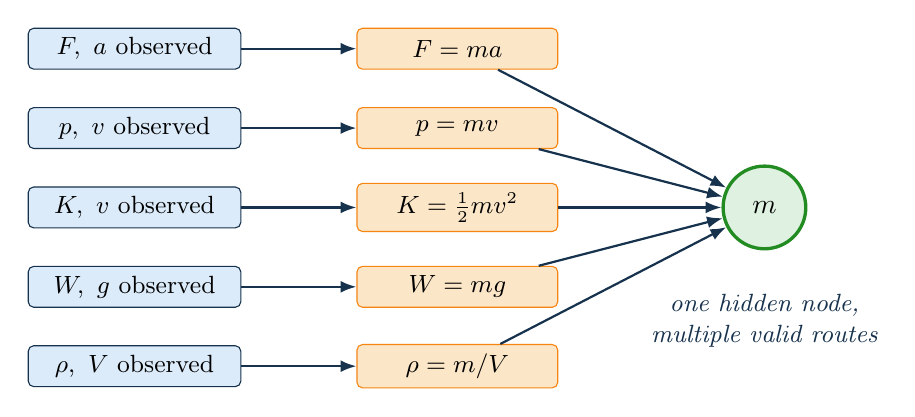
\begin{tikzpicture}[
  x=1cm,y=0.72cm,
  obs/.style={draw=ink,rounded corners=2pt,fill=nodeblue,minimum width=2.7cm,minimum height=0.52cm,align=center,font=\small},
  eq/.style={draw=BurntOrange,rounded corners=2pt,fill=edgeorange,minimum width=2.55cm,minimum height=0.52cm,align=center,font=\small},
  target/.style={circle,draw=ForestGreen,very thick,fill=lawgreen,minimum size=1.05cm,font=\bfseries},
  arr/.style={-{Latex[length=2mm]},thick,draw=ink}
]
\node[obs] (o1) at (0,2.8) {$F,\ a$ observed};
\node[obs] (o2) at (0,1.4) {$p,\ v$ observed};
\node[obs] (o3) at (0,0) {$K,\ v$ observed};
\node[obs] (o4) at (0,-1.4) {$W,\ g$ observed};
\node[obs] (o5) at (0,-2.8) {$\rho,\ V$ observed};
\node[eq] (e1) at (4.1,2.8) {$F=ma$};
\node[eq] (e2) at (4.1,1.4) {$p=mv$};
\node[eq] (e3) at (4.1,0) {$K=\tfrac12 mv^2$};
\node[eq] (e4) at (4.1,-1.4) {$W=mg$};
\node[eq] (e5) at (4.1,-2.8) {$\rho=m/V$};
\node[target] (m) at (8,0) {$m$};
\foreach \a/\b in {o1/e1,o2/e2,o3/e3,o4/e4,o5/e5} \draw[arr] (\a)--(\b);
\foreach \a in {e1,e2,e3,e4,e5} \draw[arr] (\a)--(m);
\node[align=center,font=\small\itshape,text=ink] at (8,-2.0) {one hidden node,\\multiple valid routes};
\end{tikzpicture}
\caption{The motivating idea. Depending on which quantities are observed, mass can be reached through different equation nodes. The implemented graph generalizes this pattern across 159 shared quantities.}
\label{fig:massroutes}
\end{figure}

\section{Scenario-consistent worlds}

The generator samples 13 scenario families: linear and projectile motion, circular motion, inclines, work/energy, collisions, rotation, gravitation, simple harmonic motion, fluids, thermodynamics, waves, and properties of matter. Each world is completed using the relevant equations, and representative identities are checked numerically before data are written. The corpus contains 650,000 worlds.

Magnitudes and signs are stored separately:
\begin{equation}
 \operatorname{mag}(x)=\log_{10}(|x|+10^{-12})/10 .
\end{equation}
This makes multiplication approximately additive in representation space: for example, $F=ma$ implies $\operatorname{mag}(F)\simeq\operatorname{mag}(m)+\operatorname{mag}(a)$. Additive physical equations remain nonlinear in this representation.

During training, present physical constants and a random 30--80\% of the other present quantities are revealed. Hidden quantities are reconstruction targets. Five exact input--target combinations are protected from training and generated afresh for a 7,500-example ladder exam (1,500 per route):
\begin{align*}
L0:&\ (f,r)\rightarrow v_{\tan},&
L1:&\ (T,r)\rightarrow v_{\tan},\\
L2:&\ (T,r,m)\rightarrow K,&
L3:&\ (k,m,A)\rightarrow v_{\max},\\
L4:&\ (\lambda,f,\mu)\rightarrow T_{\mathrm{tension}}.&
\end{align*}
The final test must combine $v=f\lambda$ with the inverse of $v=\sqrt{T/\mu}$.

\section{Operator-conditioned graph solver}

The solver has eight graph-attention layers, 128-dimensional states, four heads, and eight relation bases. For edge $e_{ij}$, its 16 features select a mixture of learned transforms:
\begin{equation}
 m_{ij}=\sum_{b=1}^{8}c_b(e_{ij})V_bh_j .
 \label{eq:message}
\end{equation}
Thus a value crossing a multiplication edge need not be processed like one crossing an addition, trigonometric, or reverse edge. Multi-head attention aggregates incoming messages; feed-forward residual blocks update all 305 nodes. Separate heads predict normalized magnitude and sign. Training uses Huber magnitude loss plus sign cross-entropy. The archived model has 2,165,699 parameters.

\section{Held-out routes and non-graph controls}

Table~\ref{tab:ladder} reports the immutable archived history. At epoch 40, the single archived GNN run exceeds $R^2=0.985$ on all five held-out routes. Its best validation magnitude MAE is 0.02356 at epoch 37; epoch 40 has validation MAE 0.02386 and sign accuracy 98.67\%.

\begin{table}[H]
\centering\small
\begin{tabular}{lccccc}
\toprule
 & L0 & L1 & L2 & L3 & L4\\
\midrule
GNN, epoch 0  & 0.837 & 0.511 & 0.289 & 0.559 & 0.033\\
GNN, epoch 10 & 0.983 & 0.968 & 0.778 & 0.942 & 0.927\\
GNN, epoch 40 & 0.990 & 0.994 & 0.986 & 0.991 & 0.986\\
\bottomrule
\end{tabular}
\caption{Held-out route $R^2$ from \texttt{v9\_history.json}. The GNN values come from one archived seed and are not presented as multi-seed estimates.}
\label{tab:ladder}
\end{table}

To test whether ordinary function approximation is sufficient, I train a 1,916,637-parameter flat MLP from seeds 7, 17, and 29, close to the GNN's 2,165,699 parameters. Its input is the concatenation of 159 revealed magnitudes, 159 revealed signs, and the 159-bit reveal mask. It receives the same training split, mask distribution, and ban protection as the GNN, but no graph, structural features, equation/law nodes, or scenario identity. Each seed runs for five epochs; its checkpoint is selected only by magnitude MAE on a fixed 10,000-world validation subset, after which the ladder is evaluated once. Table~\ref{tab:baselines} also includes a target-mean reference and an analytic oracle that is directly given the five formulas.

\begin{table}[H]
\centering\small
\setlength{\tabcolsep}{5pt}
\begin{tabular}{lccccc}
\toprule
Method & L0 & L1 & L2 & L3 & L4\\
\midrule
Target mean & -0.001 & -0.000 & -0.036 & -0.002 & -0.001\\
Flat MLP, 3 seeds & $0.968\pm0.006$ & $0.925\pm0.068$ & $0.877\pm0.020$ & $0.870\pm0.056$ & $0.515\pm0.060$\\
Archived GNN, 1 seed & 0.990 & 0.994 & 0.986 & 0.991 & 0.986\\
Analytic formula oracle & 1.000 & 1.000 & 1.000 & 1.000 & 1.000\\
\bottomrule
\end{tabular}
\caption{Held-out route $R^2$. MLP entries are mean $\pm$ population standard deviation across three seeds. The GNN and MLP seed counts differ, so the table is a controlled architectural reference, not a completed multi-seed GNN comparison.}
\label{tab:baselines}
\end{table}

\section{Do node and edge features matter?}

I intervene on the archived best checkpoint at inference time using a deterministic 100-example subset of each route. One feature group is zeroed at a time; the last condition removes all reverse edges. Table~\ref{tab:ablations} shows that the full checkpoint remains strong, while removing structural information often causes severe degradation. In particular, edge roles are essential on the longer routes, and reverse edges are important for the inversion-heavy L4 test.

\begin{table}[H]
\centering\scriptsize
\setlength{\tabcolsep}{4.2pt}
\begin{tabular}{lrrrrrr}
\toprule
Inference condition & L0 & L1 & L2 & L3 & L4 & Aggregate MAE\\
\midrule
Full checkpoint & .997 & .994 & .990 & .990 & .964 & .0084\\
Zero node SI dimensions & .955 & .825 & .521 & .565 & .177 & .0521\\
Zero node semantics & .805 & .860 & .635 & .942 & -.791 & .0538\\
Zero edge operators & .696 & .195 & .170 & .124 & .244 & .0742\\
Zero edge role/direction & .514 & .529 & -1.095 & -.908 & -18.387 & .1465\\
Zero edge flags & .870 & .921 & .591 & .899 & .973 & .0358\\
Remove reverse edges & .917 & .353 & .301 & .878 & -1.755 & .0683\\
\bottomrule
\end{tabular}
\caption{Diagnostic interventions on one already-trained checkpoint. Columns L0--L4 are $R^2$; MAE is in normalized log-magnitude units. These distribution-shifting interventions do not replace independent retraining of each ablated architecture.}
\label{tab:ablations}
\end{table}

The test supports a limited but important conclusion: the archived solver's predictions depend on both what a node represents and what an edge instructs. It does not by itself establish causal importance during training, because the ablated models were not retrained.

\section{Mine, then prove}

After training, the miner examines ordered pairs of distant quantity nodes $(A,B)$. It reveals $A$ and applicable constants, sweeps $A$ in log-magnitude space, and records the predicted response at $B$. A near-linear response with slope $k$ proposes a local hypothesis $B\propto A^k$.

The audit then converts every monomial equation into an exact linear constraint over log-magnitudes. Rational Gaussian elimination either returns a formula with a proof trace or declines to certify it. Unproved candidates are evaluated under regenerated distributions with altered sampling ranges; a slope that changes under this prior shift is treated as a sampling artifact. Additive and trigonometric routes are explicitly outside the current monomial certifier.

The 400-pair screen contains 12 proven-pure and 242 proven-conditional entries (254 unique certified formulas), 33 prior-sensitive artifacts, 91 additive-mediated cases, 6 unresolved-invariant cases, and 16 unresolved cases. Familiar corollaries such as $v_{\mathrm{esc}}=\sqrt{2}v_{\mathrm{orb}}$ and $PE_{\mathrm{orb}}=2E_{\mathrm{orb}}$ are useful rediscoveries, not new laws.

\section{Author perspective, mission, and real data}

I grew up in a low-income family in Bihar and have not had the money, laboratory access, or instruments needed to collect a broad real-world physics dataset. That constraint shaped this first study. A synthetic corpus made it possible to build and test the reasoning pipeline with ordinary computing resources, and its closed nature provides a strong audit: if the system claims unknown physics here, the claim must be rejected.

Synthetic success is only a beginning. Real measurements contain noise, calibration error, selection effects, hidden variables, and model mismatch---exactly the difficulties a discovery system must survive. The next stage should use independently collected datasets, freeze evaluation protocols before fitting, compare against symbolic and numerical solvers, and require a candidate relation to replicate across instruments or laboratories.

My long-term mission is to teach an AI physics deeply enough that it can combine more paths and evidence than any one person can hold at once, and eventually help humans find genuinely new physics. That is an aspiration, not a result of this paper. The present contribution is a small, inspectable step: teach a model to navigate known physics, then make it prove what it can and admit what it cannot.

\section{Limitations and claim boundary}

The corpus is synthetic, closed, and generated from the encoded equations. It establishes neither experimental validity nor a new physical law. The GNN has one archived training seed; the MLP baseline has three seeds and is a fixed five-epoch reference rather than an exhaustive hyperparameter study; the checkpoint interventions are not retrained ablations. The graph and generator contain modeling choices that can induce correlations. The certifier currently handles monomial algebra but not general additive or trigonometric derivations. No comparison is yet made against a complete symbolic equation solver under identical masking.

Accordingly, the defensible claims are that the archived model predicts five protected routes accurately, that a similarly sized flat network provides a weaker or different reference on those routes, that the trained checkpoint is sensitive to designed node and edge information, and that the audit prevents rediscovered encoded relationships from being presented as novel physics.

\section*{Reproducibility and disclosure}

Code, graph construction, data generation, the immutable training history, checkpoint diagnostics, multi-seed baseline output, discovery audit, hashes, and an exact CPU environment lock are available in the
\href{https://github.com/mi99at/physics-gnn-symbolic-discovery}{project repository}
and archived under the stable concept DOI
\href{https://doi.org/10.5281/zenodo.21984785}{10.5281/zenodo.21984785}.
Large arrays and checkpoints are stored in the archival release rather than Git. Drafting, editing, and coding used AI assistance. The author directed the project and is responsible for its design, experiments, interpretation, and final text.

\begin{thebibliography}{9}\footnotesize
\setlength{\itemsep}{1pt}
\bibitem{gilmer2017} J. Gilmer et al. Neural message passing for quantum chemistry. \emph{ICML}, 2017.
\bibitem{kipf2017} T. Kipf and M. Welling. Semi-supervised classification with graph convolutional networks. \emph{ICLR}, 2017.
\bibitem{velickovic2018} P. Veli\v{c}kovi\'c et al. Graph attention networks. \emph{ICLR}, 2018.
\bibitem{battaglia2018} P. Battaglia et al. Relational inductive biases, deep learning, and graph networks. arXiv:1806.01261, 2018.
\bibitem{schlichtkrull2018} M. Schlichtkrull et al. Modeling relational data with graph convolutional networks. \emph{ESWC}, 2018.
\bibitem{udrescu2020} S.-M. Udrescu and M. Tegmark. AI Feynman. \emph{Science Advances}, 2020.
\bibitem{cranmer2023} M. Cranmer. Interpretable machine learning for science with PySR. arXiv:2305.01582, 2023.
\bibitem{raissi2019} M. Raissi, P. Perdikaris, and G. Karniadakis. Physics-informed neural networks. \emph{Journal of Computational Physics}, 2019.
\end{thebibliography}

\end{document}
